% --- 仅输入正文内容 ---

\section{实验目的}

\begin{enumerate}[label=\arabic*、, leftmargin=4em, labelsep=0pt]
    \item 学习四探针法测量半导体材料电阻率的基本原理；
    \item 掌握 RTS-9 型四探针测试仪的操作方法；
    \item 学会使用四探针法测量薄膜材料的方块电阻和电阻率；
    \item 理解修正因子 $K$ 和厚度修正因子 $F(W/S)$ 的物理意义。
\end{enumerate}

\section{实验原理（简述）}

\subsection{四探针法基本原理}

四探针法将四根等间距金属探针压在样品表面，外侧探针（1、4号）通恒定电流 $I$，内侧探针（2、3号）测电位差 $V$。对半无穷大样品，电阻率：
\begin{equation}
    \rho = 2\pi S \cdot \frac{V}{I}
\end{equation}
其中探针间距 $S = 1$ mm。

\subsection{两种测量组合与计算公式}

RTS-9 型四探针测试仪支持两种模式，均通过正反向测量取平均以消除热电势干扰：

\begin{enumerate}[label=\arabic*、, leftmargin=4em, labelsep=0pt]
    \item \textbf{$I_{14}V_{23}$ 模式}：$V_{23} = (V_{23+} + V_{23-})/2$
    \item \textbf{$I_{13}V_{24}$ 模式}：$V_{24} = (V_{24+} + V_{24-})/2$
\end{enumerate}

先计算比值 $V_{23}/V_{24}$，查表得修正因子 $K$，则：

\textbf{方块电阻}（$\Omega/\square$）：$R_{\square} = K \cdot V_{23}/I$

\textbf{电阻率}（$\Omega \cdot \text{cm}$）：$\rho = R_{\square} \cdot W \cdot F(W/S) \times 10^{-1}$，其中 $W$ 为厚度，$F(W/S)$ 为厚度修正因子（$W/S < 0.5$ 时需修正）。

\subsection{实验仪器}

RTS-9 型四探针测试仪由四探针探头（碳化钨探针，间距 1 mm，可升降）、恒流源（10 $\mu$A $\sim$ 100 mA 连续可调）、高输入阻抗数字电压表、样品台及计算机专用测试软件组成。前面板含电源开关、电流调节旋钮、电流/电压显示窗口、模式选择开关及探针升降旋钮。

\section{实验内容及步骤}

四探针法测量电阻率的基本操作流程如下：

\begin{enumerate}[label=\arabic*、, leftmargin=4em, labelsep=0pt]
    \item \textbf{开机预热}：打开 RTS-9 测试仪电源，预热 15--20 分钟至稳定状态；
    \item \textbf{启动软件}：运行 RTS-9 专用测试软件，进入测试主界面；
    \item \textbf{放置样品}：将样品置于样品台上，确保表面平整、洁净，待测区域位于探针正下方；
    \item \textbf{设置参数}：在"测试基本参数窗口"输入样品厚度 $W$、探针间距 $S$（1 mm），并选择适当测试电流；
    \item \textbf{调节电流}：旋转电流调节旋钮至目标值（如 45.32 $\mu$A），确认；
    \item \textbf{降下探针}：旋转探针升降旋钮使四根探针与样品良好接触（力度适中）；
    \item \textbf{采集数据}：软件实时显示 $V_{23+}$、$V_{23-}$、$V_{24+}$、$V_{24-}$；
    \item \textbf{统计数据}：点击"统计测试数据"，软件自动计算 $V_{23}$、$V_{24}$、比值 $V_{23}/V_{24}$、修正因子 $K$、方块电阻 $R_{\square}$ 及电阻率 $\rho$；
    \item \textbf{记录并多点测量}：记录数据，升起探针，移动样品至新位置，重复步骤 6--8，至少测量 5 个点；
    \item \textbf{结束实验}：升起探针，关闭软件和仪器电源，整理实验台。
\end{enumerate}

软件操作栏提供开始/停止测试、保存/打开数据及打印报告等功能。

\section{实验结果及数据分析}

\subsection{样品信息}

\begin{table}[H]
    \centering
    \caption{待测样品信息}
    \begin{tabular}{p{2cm}p{3cm}p{2cm}p{2.5cm}p{2.5cm}}
        \toprule
        样品编号 & 样品描述 & 厚度 $W$(mm) & 测试电流 $I$(mA) & 修正系数 $F$ \\
        \midrule
        001SI & 硅片 & 0.50 & 0.9999 & 0.9975 \\
        001cu & 铜薄膜 & 0.10 & 99.97 & 1.0000 \\
        \bottomrule
    \end{tabular}
\end{table}

实验条件：温度 30$^\circ$C，相对湿度 52\%RH，探针间距 $S = 1.00$ mm。

\subsection{样品一：硅片（001SI）测量数据}

\begin{table}[H]
    \centering
    \caption{硅片四探针测量数据记录表（$I = 0.9999$ mA，$W = 0.50$ mm）}
    \begin{tabular}{ccccccc}
        \toprule
        测量点 & $V_{23+}$(mV) & $V_{23-}$(mV) & $V_{24+}$(mV) & $V_{24-}$(mV) & $V_{23}$(mV) & $V_{24}$(mV) \\
        \midrule
        1 & 5.50 & 5.53 & 4.19 & 4.46 & 5.515 & 4.325 \\
        2 & 5.50 & 5.53 & 4.43 & 4.46 & 5.515 & 4.445 \\
        3 & 5.50 & 5.53 & 4.42 & 4.47 & 5.515 & 4.445 \\
        4 & 5.50 & 5.53 & 4.43 & 4.47 & 5.515 & 4.450 \\
        5 & 5.50 & 5.54 & 4.40 & 4.47 & 5.520 & 4.435 \\
        6 & 5.50 & 5.54 & 4.43 & 4.47 & 5.520 & 4.450 \\
        7 & 5.49 & 5.54 & 4.41 & 4.48 & 5.515 & 4.445 \\
        \bottomrule
    \end{tabular}
\end{table}

\subsection{样品二：铜薄膜（001cu）测量数据}

\begin{table}[H]
    \centering
    \caption{铜薄膜四探针测量数据记录表（$I = 99.97$ mA，$W = 0.10$ mm）}
    \begin{tabular}{ccccccc}
        \toprule
        测量点 & $V_{23+}$(mV) & $V_{23-}$(mV) & $V_{24+}$(mV) & $V_{24-}$(mV) & $V_{23}$(mV) & $V_{24}$(mV) \\
        \midrule
        1 & 0.024 & 0.026 & 0.019 & 0.020 & 0.0250 & 0.0195 \\
        2 & 0.024 & 0.026 & 0.019 & 0.020 & 0.0250 & 0.0195 \\
        3 & 0.024 & 0.026 & 0.019 & 0.020 & 0.0250 & 0.0195 \\
        4 & 0.024 & 0.026 & 0.020 & 0.020 & 0.0250 & 0.0200 \\
        5 & 0.024 & 0.026 & 0.020 & 0.020 & 0.0250 & 0.0200 \\
        \bottomrule
    \end{tabular}
\end{table}

\subsection{计算结果汇总}

\begin{table}[H]
    \centering
    \caption{两种样品电阻率计算结果对比}
    \begin{tabular}{cccccc}
        \toprule
        样品 & 测量点数 & $\rho_{\max}$ & $\rho_{\min}$ & $\rho_{\text{avg}}$ & 电阻率单位 \\
        \midrule
        硅片 (001SI) & 7 & 1.27 & 1.21 & 1.226 & $\Omega \cdot \text{cm}$ \\
        铜薄膜 (001cu) & 5 & 11.6 & 11.2 & 11.44 & $\mu\Omega \cdot \text{cm}$ \\
        \bottomrule
    \end{tabular}
\end{table}

\subsection{数据分析}

\begin{enumerate}[label=\arabic*、, leftmargin=4em, labelsep=0pt]
    \item \textbf{电阻率均匀性评价}：\\
    硅片不均匀度：
    $\Delta_{\text{Si}} = \dfrac{1.27 - 1.21}{1.226} \times 100\% \approx 4.89\%$；\\
    铜薄膜不均匀度：
    $\Delta_{\text{Cu}} = \dfrac{11.6 - 11.2}{11.44} \times 100\% \approx 3.50\%$。\\
    两种样品的不均匀度均小于 5\%，表明样品电阻率分布较为均匀，其中铜薄膜的均匀性优于硅片。
    
    \item \textbf{数据可靠性分析}：硅片测量 7 个点、铜薄膜测量 5 个点，各点数据偏差较小，无异常数据点，测量结果具有较好的重复性和可靠性。
    
    \item \textbf{厚度修正分析}：硅片 $W/S = 0.5$，修正系数 $F = 0.9975$，修正幅度较小（约 0.25\%）；铜薄膜 $W/S = 0.1$（远小于 0.5），但因修正系数 $F = 1.0000$，说明对于高导电金属薄膜，在一定条件下厚度修正影响有限。
    
    \item \textbf{材料特性对比}：硅片电阻率约 1.226 $\Omega \cdot \text{cm}$，属典型半导体材料；铜薄膜电阻率约 11.44 $\mu\Omega \cdot \text{cm}$（$1.144 \times 10^{-6}\,\Omega \cdot \text{cm}$），接近纯铜体电阻率（$1.68\,\mu\Omega \cdot \text{cm}$），表明铜薄膜具有良好的导电性。
\end{enumerate}

\section{实验结论}

\begin{enumerate}[label=\arabic*、, leftmargin=4em, labelsep=0pt]
    \item 本次实验采用 RTS-9 型四探针测试仪，对硅片（001SI）和铜薄膜（001cu）两种样品进行了电阻率测量，成功获得了可靠的实验数据；
    \item 硅片电阻率平均值 $\rho_{\text{Si}} = 1.226\ \Omega \cdot \text{cm}$（7 点测量，不均匀度 4.89\%），属典型半导体电阻率范围；
    \item 铜薄膜电阻率平均值 $\rho_{\text{Cu}} = 11.44\ \mu\Omega \cdot \text{cm}$（5 点测量，不均匀度 3.50\%），接近纯铜体电阻率理论值，导电性良好；
    \item 两种样品的不均匀度均小于 5\%，表明测量结果重复性好，四探针法能有效消除接触电阻和热电势的影响；
    \item 厚度修正因子 $F(W/S)$ 对硅片（$W/S = 0.5$）有约 0.25\% 的微小修正，实践中不可忽略。
\end{enumerate}

\section{实验注意事项}

\begin{enumerate}[label=\arabic*、, leftmargin=4em, labelsep=0pt]
    \item 测试前确保样品表面清洁，无氧化层或污染，否则会影响接触电阻；
    \item 探针与样品接触力度适中，过大会损伤探针或样品，过小会导致接触不良；
    \item 每次测量前等待电流和电压读数稳定后再记录数据；
    \item 高阻样品应注意电磁屏蔽，避免外界干扰；
    \item 测试电流不宜过大，避免焦耳热效应导致电阻率变化；
    \item 测量薄膜样品时，确保基底为绝缘材料，避免漏电流；
    \item 实验结束后务必升起探针，避免探针长时间受压变形。
\end{enumerate}

\section{附教师签字版实验数据表}

\begin{figure}[H]
    \centering
    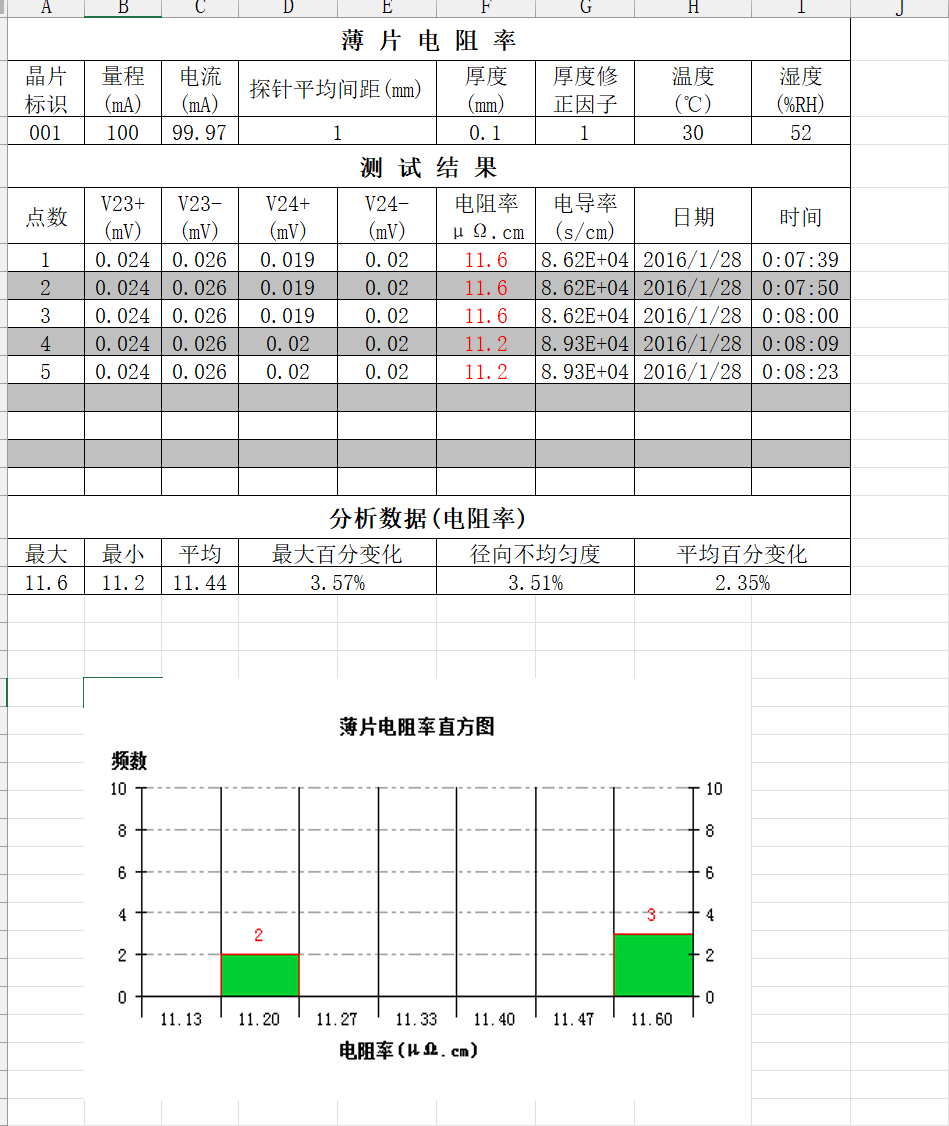
\includegraphics[width=0.85\textwidth]{pictures/image.png}
    \caption{硅片（001SI）原始实验数据表（$I = 1$ mA，$W = 0.50$ mm）}
    \label{fig:datasheet-si}
\end{figure}

\begin{figure}[H]
    \centering
    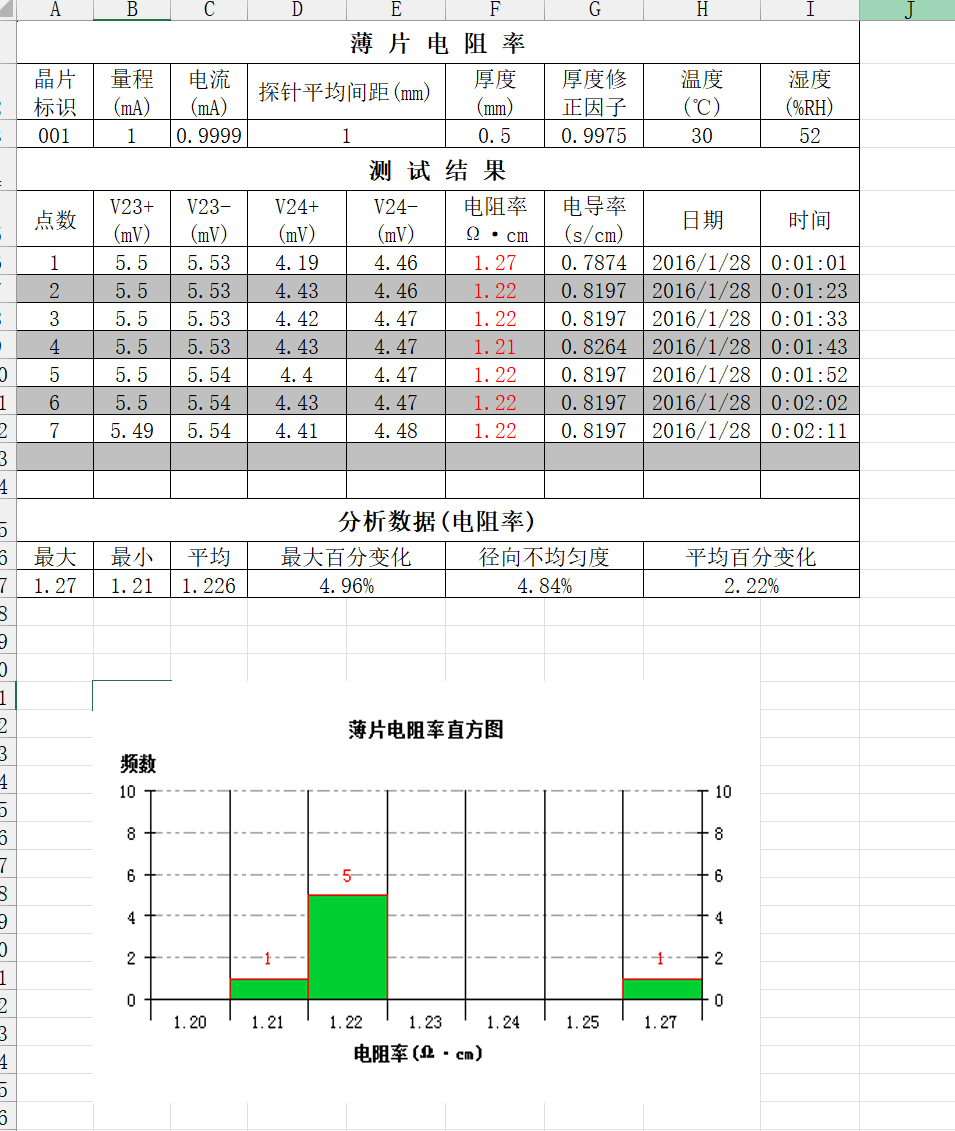
\includegraphics[width=0.85\textwidth]{pictures/屏幕截图 2026-06-19 221122.png}
    \caption{铜薄膜（001cu）原始实验数据表（$I = 100$ mA，$W = 0.10$ mm）}
    \label{fig:datasheet-cu}
\end{figure}